\documentclass[aspectratio=169, 10pt]{beamer}

\usetheme{Madrid}
\usecolortheme{whale}

\usepackage{amsmath, amssymb, amsthm}
\usepackage{bm}
\usepackage{tikz}
\usetikzlibrary{arrows.meta, positioning, shapes.geometric, fit, backgrounds}
\usepackage{booktabs}
\usepackage{xcolor}
\usepackage{multirow}
\usepackage{array}

% Custom colors
\definecolor{darkblue}{RGB}{0,51,102}
\definecolor{darkred}{RGB}{153,0,0}
\definecolor{darkgreen}{RGB}{0,102,51}
\definecolor{lightorange}{RGB}{255,240,210}
\definecolor{lightblue}{RGB}{220,235,245}
\definecolor{lightyellow}{RGB}{255,250,220}
\definecolor{lightgreen}{RGB}{220,245,220}
\definecolor{lightred}{RGB}{245,220,220}
\definecolor{medblue}{RGB}{100,149,200}

\setbeamercolor{palette primary}   {bg=darkblue, fg=white}
\setbeamercolor{palette secondary} {bg=darkblue!80, fg=white}
\setbeamercolor{palette tertiary}  {bg=darkblue!60, fg=white}
\setbeamercolor{palette quaternary}{bg=darkblue, fg=white}
\setbeamercolor{frametitle}        {bg=darkblue, fg=white}
\setbeamercolor{title}             {fg=white}

%
%===================================================================================================
%
% Title page information

\author{Giovanni Della Lunga\\{\footnotesize giovanni.dellalunga@unibo.it}}
\title{Chapter 2\\Factor Models and Dimensionality Reduction}
\subtitle{Appendix 2 - Firm Characteristics in Asset Pricing} % (optional)
\setbeamercovered{transparent} 
\institute{Advanced Topics in Artificial Intelligence} 
\date{Bologna - March, 2026} 



\begin{document}

% -------------------------------------------------------
\begin{frame}
\titlepage
\end{frame}

% -------------------------------------------------------
\begin{frame}{Roadmap}
\tableofcontents
\end{frame}

% -------------------------------------------------------
\section{Motivation: Why Characteristics?}
%
%..................................................................
%
\begin{frame}{The Problem with Static Betas — A Concrete Example}

Consider two firms at the \textbf{same point in time}:

\begin{center}
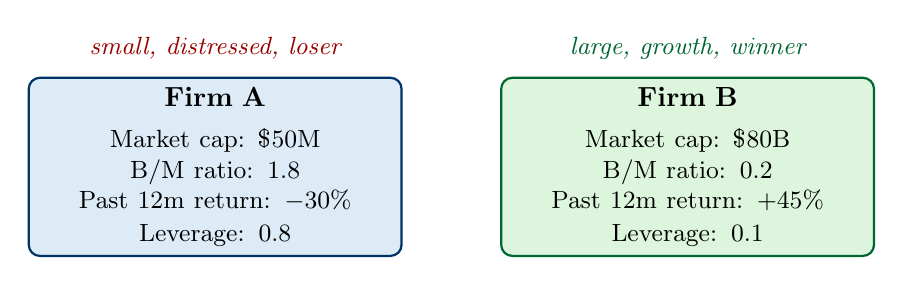
\begin{tikzpicture}
  \node[rectangle, rounded corners, draw=darkblue, thick, fill=lightblue,
        text width=4.5cm, align=center, minimum height=2.2cm] (A) at (0,0) {
    \textbf{Firm A} \\[4pt]
    \small Market cap: \$50M \\
    \small B/M ratio: 1.8 \\
    \small Past 12m return: $-30\%$ \\
    \small Leverage: 0.8
  };
  \node[rectangle, rounded corners, draw=darkgreen, thick, fill=lightgreen,
        text width=4.5cm, align=center, minimum height=2.2cm] (B) at (6,0) {
    \textbf{Firm B} \\[4pt]
    \small Market cap: \$80B \\
    \small B/M ratio: 0.2 \\
    \small Past 12m return: $+45\%$ \\
    \small Leverage: 0.1
  };
  \node[above=0.1cm of A, font=\small\itshape, text=darkred]
        {small, distressed, loser};
  \node[above=0.1cm of B, font=\small\itshape, text=darkgreen]
        {large, growth, winner};
\end{tikzpicture}
\end{center}

\bigskip
\textbf{Key question:} should Firm A and Firm B have the \emph{same} market beta? 
The \emph{same} sensitivity to a recession shock?

\medskip
\begin{alertblock}{The static model assumption}
In static factor models (FF, PCA), $\beta_i$ is \textbf{constant} for each firm.
Both firms get a single number estimated from 60 months of past returns.
This ignores all the information in their current observable attributes.
\end{alertblock}

\end{frame}
%
%..................................................................
%
\begin{frame}{Characteristics as Signals of Risk Exposure}

Economic theory and empirical evidence suggest that \textbf{observable firm attributes
predict how a firm responds to systematic shocks}:

\bigskip
\begin{center}
\begin{tabular}{p{3.2cm} p{4.5cm} p{4.5cm}}
\toprule
\textbf{Characteristic} & \textbf{Economic rationale} & \textbf{Expected effect on $\beta$} \\
\midrule
\textbf{Size} (market cap)
  & Small firms more exposed to liquidity and credit shocks
  & Small $\Rightarrow$ higher distress $\beta$ \\[6pt]
\textbf{Value} (B/M ratio)
  & High B/M firms have more assets in place, less flexibility
  & High B/M $\Rightarrow$ higher value $\beta$ \\[6pt]
\textbf{Momentum} (past returns)
  & Recent winners differ in investor attention, short-sale pressure
  & High mom $\Rightarrow$ different factor loading \\[6pt]
\textbf{Leverage}
  & More debt amplifies equity sensitivity to macro shocks
  & High lev $\Rightarrow$ higher market $\beta$ \\[6pt]
\textbf{Profitability}
  & Profitable firms less exposed to financial distress
  & High prof $\Rightarrow$ lower crash $\beta$ \\
\bottomrule
\end{tabular}
\end{center}
\end{frame}
%
%..................................................................
%
\begin{frame}{Characteristics as Signals of Risk Exposure}
\begin{block}{The key insight}
Characteristics are \textbf{proxies for latent risk exposures}. They contain information
about $\beta$ that is not captured by past returns alone.
\end{block}

\end{frame}

% -------------------------------------------------------
\section{What Are Firm Characteristics?}
%
%..................................................................
%
\begin{frame}{Definition: Firm Characteristics}

\begin{block}{Definition}
A \textbf{firm characteristic} $z_{i,p,t-1}$ is any observable attribute of firm $i$,
measured at time $t-1$, that carries information about its future returns or risk
exposures.
\end{block}

\bigskip
Characteristics are collected into a vector for each firm and period:

$$z_{i,t-1} = \begin{pmatrix} z_{i,1,t-1} \\ z_{i,2,t-1} \\ \vdots \\ z_{i,P,t-1} \end{pmatrix} \in \mathbb{R}^P$$

\medskip
They come from \textbf{different data sources}, updated at different frequencies:

\begin{center}
\begin{tabular}{lcl}
\toprule
\textbf{Source} & \textbf{Frequency} & \textbf{Examples} \\
\midrule
Financial statements & Annual / Quarterly & B/M, leverage, profitability, investment \\
Market data         & Monthly            & Size, momentum, volatility, liquidity \\
\bottomrule
\end{tabular}
\end{center}

%\medskip
%In the paper (Gu, Kelly, Xiu 2020): $P = 94$ characteristics per firm per month.

\end{frame}
%
%..................................................................
%
\begin{frame}{Categories of Characteristics}

\begin{center}
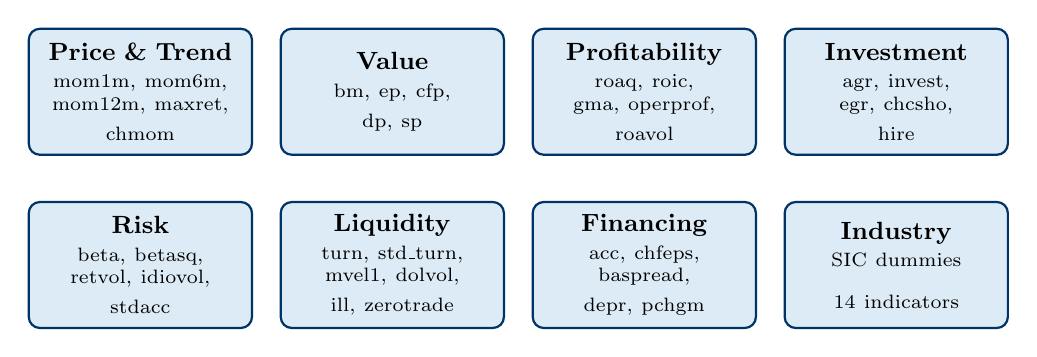
\begin{tikzpicture}[
  cat/.style={rectangle, rounded corners, draw=darkblue, thick,
              fill=lightblue, text width=2.6cm, align=center,
              minimum height=1.6cm, font=\small},
  item/.style={font=\scriptsize, align=left}
]

\node[cat] (pt) at (0, 2.2)   {\textbf{Price \& Trend}\\[2pt]\scriptsize mom1m, mom6m,\\ mom12m, maxret,\\ chmom};
\node[cat] (va) at (3.2, 2.2) {\textbf{Value}\\[2pt]\scriptsize bm, ep, cfp,\\ dp, sp};

\node[cat] (pr) at (6.4, 2.2) {\textbf{Profitability}\\[2pt]\scriptsize roaq, roic,\\ gma, operprof,\\ roavol};
\node[cat] (in) at (9.6, 2.2) {\textbf{Investment}\\[2pt]\scriptsize agr, invest,\\ egr, chcsho,\\ hire};

\node[cat] (ri) at (0, 0)     {\textbf{Risk}\\[2pt]\scriptsize beta, betasq,\\ retvol, idiovol,\\ stdacc};
\node[cat] (lq) at (3.2, 0)   {\textbf{Liquidity}\\[2pt]\scriptsize turn, std\_turn,\\ mvel1, dolvol,\\ ill, zerotrade};
\node[cat] (fi) at (6.4, 0)   {\textbf{Financing}\\[2pt]\scriptsize acc, chfeps,\\ baspread,\\ depr, pchgm};
\node[cat] (in2) at (9.6, 0)  {\textbf{Industry}\\[2pt]\scriptsize SIC dummies\\[4pt]\scriptsize 14 indicators};

%\node[above=0.05cm of pt, font=\tiny\itshape, text=darkred]  %{20 chars};
%\node[above=0.05cm of va, font=\tiny\itshape, text=darkred]  %{14 chars};
%\node[above=0.05cm of pr, font=\tiny\itshape, text=darkred]  %{13 chars};
%\node[above=0.05cm of in, font=\tiny\itshape, text=darkred]  %{10 chars};
%\node[below=0.05cm of ri,  font=\tiny\itshape, text=darkred] %{9 chars};
%\node[below=0.05cm of lq,  font=\tiny\itshape, text=darkred] %{7 chars};
%\node[below=0.05cm of fi,  font=\tiny\itshape, text=darkred] %{7 chars};
%\node[below=0.05cm of in2, font=\tiny\itshape, text=darkred] %{14 chars};
\end{tikzpicture}
\end{center}

\medskip
%\begin{exampleblock}{Update frequencies}
%61 annual \quad $|$ \quad 13 quarterly \quad $|$ \quad 20 monthly
%\end{exampleblock}

\end{frame}
%
%..................................................................
%
\begin{frame}{Preprocessing: Rank Normalization}

Raw characteristics are \textbf{not} used directly. They are preprocessed to ensure
comparability across firms and over time.

\bigskip
\textbf{Procedure for each characteristic $p$ at each date $t$:}

\begin{enumerate}
  \item \textbf{Cross-sectional rank:} for each date $t$, rank all $N_t$ firms by
        characteristic $p$
        $$\text{rank}_{i,p,t} \in \{1, 2, \ldots, N_t\}$$

  \item \textbf{Normalize} to the interval $(-1, +1)$:
        $$\tilde{z}_{i,p,t} = 2\cdot\frac{\text{rank}_{i,p,t} - 1}{N_t - 1} - 1$$
\end{enumerate}
\end{frame}
%
%..................................................................
%
\begin{frame}{Preprocessing: Rank Normalization}
\begin{columns}
\begin{column}{0.48\textwidth}
  \begin{alertblock}{Why rank normalization?}
    \begin{itemize}
      \item Eliminates \textbf{outliers} (e.g.\ extreme P/E ratios)
      \item Makes all characteristics \textbf{comparable} in scale
      \item Removes distributional changes over time
      \item Standard in empirical asset pricing ML
    \end{itemize}
  \end{alertblock}
\end{column}
\begin{column}{0.48\textwidth}
  \begin{exampleblock}{Example}
    \small If there are 3000 firms and Apple ranks 2700th by size,
    its normalized size characteristic is:
    $$\tilde{z} = 2\cdot\frac{2699}{2999} - 1 \approx +0.80$$
    A micro-cap ranked 50th would get $\approx -0.97$.
  \end{exampleblock}
\end{column}
\end{columns}

\end{frame}

% -------------------------------------------------------
\section{The Characteristics Panel}
%
%..................................................................
%
\begin{frame}{The Characteristics Panel: Data Structure}

For $N$ firms observed over $T$ months, each with $P$ characteristics, the full
dataset is a \textbf{three-dimensional panel}:

\bigskip
\begin{center}
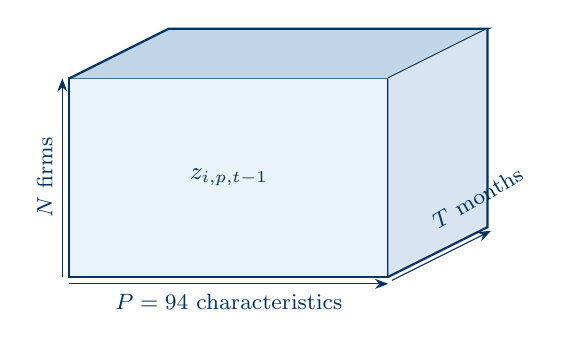
\begin{tikzpicture}[scale=0.9]
  % 3D box
  \def\W{4.5} \def\H{2.8} \def\D{1.4}
  % front face
  \fill[lightblue!60] (0,0) rectangle (\W,\H);
  \draw[darkblue, thick] (0,0) rectangle (\W,\H);
  % top face
  \fill[medblue!40]
    (0,\H) -- (\D,\H+\D*0.5) -- (\W+\D,\H+\D*0.5) -- (\W,\H) -- cycle;
  \draw[darkblue, thick]
    (0,\H) -- (\D,\H+\D*0.5) -- (\W+\D,\H+\D*0.5) -- (\W,\H);
  % right face
  \fill[medblue!25]
    (\W,0) -- (\W+\D,\D*0.5) -- (\W+\D,\H+\D*0.5) -- (\W,\H) -- cycle;
  \draw[darkblue, thick]
    (\W,0) -- (\W+\D,\D*0.5) -- (\W+\D,\H+\D*0.5);
  % labels
  \node[font=\small\bfseries, text=darkblue] at (\W/2, \H/2)
    {$z_{i,p,t-1}$};
  \node[font=\footnotesize, text=darkblue, rotate=90] at (-0.35, \H/2)
    {$N$ firms};
  \node[font=\footnotesize, text=darkblue] at (\W/2, -0.35)
    {$P = 94$ characteristics};
  \node[font=\footnotesize, text=darkblue, rotate=30] at (\W+\D*0.9, \H*0.4)
    {$T$ months};
  % arrows
  \draw[-{Stealth}, darkblue] (-0.1,0) -- (-0.1,\H);
  \draw[-{Stealth}, darkblue] (0,-0.1) -- (\W,-0.1);
  \draw[-{Stealth}, darkblue] (\W+0.05,-0.05) -- (\W+\D+0.05,\D*0.5-0.05);
\end{tikzpicture}
\end{center}
\end{frame}
%
%..................................................................
%
\begin{frame}{The Characteristics Panel: Data Structure}
\begin{block}{The characteristics matrix at time $t$}
For a given month $t$, we stack the characteristic vectors of all $N_t$ active firms:
$$Z_{t-1} = \begin{pmatrix} z_{1,t-1}' \\ z_{2,t-1}' \\ \vdots \\ z_{N_t,t-1}' \end{pmatrix}
\in \mathbb{R}^{N_t \times P}$$
This matrix changes every month as firms enter and exit the sample.
\end{block}

\end{frame}
%
%..................................................................
%
\begin{frame}{Time Variation: Characteristics Change Every Month}

\textbf{Apple Inc.\ (AAPL) — selected characteristics over time (illustrative):}

\begin{center}
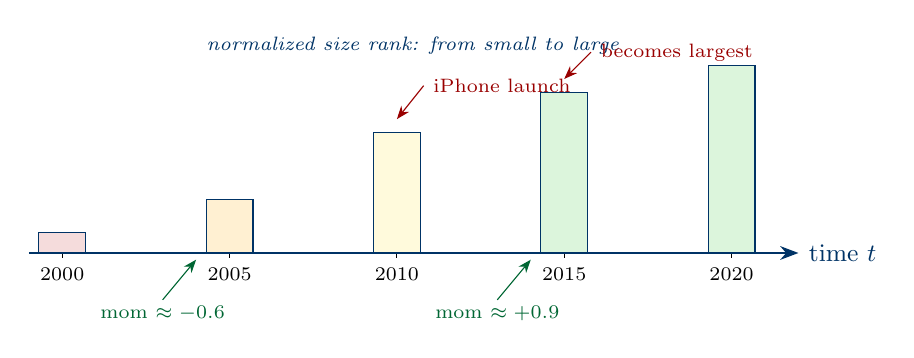
\begin{tikzpicture}[scale=0.85]
  % timeline
  \draw[-{Stealth}, thick, darkblue] (0,0) -- (11.5,0)
    node[right, font=\small] {time $t$};
  \foreach \x/\yr in {0.5/2000, 3/2005, 5.5/2010, 8/2015, 10.5/2020}
    \draw (\x, 0.08) -- (\x,-0.08) node[below, font=\scriptsize] {\yr};

  % size bar (growing)
  \foreach \x/\h/\c in {0.5/0.3/lightred, 3/0.8/lightorange,
                          5.5/1.8/lightyellow, 8/2.4/lightgreen,
                          10.5/2.8/lightgreen}
    \fill[\c, draw=darkblue] (\x-0.35,0) rectangle (\x+0.35,\h);

  \node[font=\scriptsize, text=darkblue] at (5.75, 3.1)
    {\textit{normalized size rank: from small to large}};
  \draw[{Stealth}-, darkred, thin] (5.5,2.0) -- (5.9,2.5)
    node[right, font=\scriptsize, text=darkred] {iPhone launch};
  \draw[{Stealth}-, darkred, thin] (8,2.6) -- (8.4,3.0)
    node[right, font=\scriptsize, text=darkred] {becomes largest};

  % momentum annotation
  \node[font=\scriptsize, text=darkgreen] at (2.0,-0.9)
    {mom $\approx -0.6$};
  \node[font=\scriptsize, text=darkgreen] at (7.0,-0.9)
    {mom $\approx +0.9$};
  \draw[-{Stealth}, darkgreen, thin] (2.0,-0.7) -- (2.5,-0.1);
  \draw[-{Stealth}, darkgreen, thin] (7.0,-0.7) -- (7.5,-0.1);

\end{tikzpicture}
\end{center}

\begin{block}{The implication for betas}
As Apple grew from a small struggling firm to a mega-cap growth company, its
exposure to systematic risk factors changed \textbf{continuously}. A static beta
estimated over a 5-year window cannot capture this evolution.
Characteristics provide a \textbf{real-time signal} about current risk exposure.
\end{block}

\end{frame}
%
%..................................................................
%
\begin{frame}{The Conditional Factor Model}

We now have all the ingredients to write the \textbf{general conditional factor model}:

\bigskip
\begin{alertblock}{General Conditional Factor Model (Eq.\ 1 of the paper)}
$$r_{i,t} = \beta(z_{i,t-1})'\, f_t + u_{i,t}$$
\end{alertblock}

\bigskip
\begin{center}
\begin{tabular}{cll}
\toprule
\textbf{Symbol} & \textbf{Dimension} & \textbf{Meaning} \\
\midrule
$r_{i,t}$         & scalar   & excess return of stock $i$ at time $t$ \\
$z_{i,t-1}$       & $P\times 1$ & \textbf{characteristics} of firm $i$ known at $t-1$ \\
$\beta(z_{i,t-1})$& $K\times 1$ & \textbf{conditional} factor loadings — a function of $z$ \\
$f_t$             & $K\times 1$ & latent factors at time $t$ \\
$u_{i,t}$         & scalar   & idiosyncratic return \\
\bottomrule
\end{tabular}
\end{center}
\end{frame}
%
%..................................................................
%
\begin{frame}{The Conditional Factor Model}
\begin{exampleblock}{What changed relative to the static model?}
In the static model: $\beta_i$ is a fixed vector estimated once per firm.\\
Here: $\beta(z_{i,t-1})$ is a \textbf{function} evaluated freshly every month
using the firm's current observable attributes.
\end{exampleblock}

\end{frame}
%
%..................................................................
%
\begin{frame}{How Characteristics Generate Time-Varying Betas}

\begin{center}
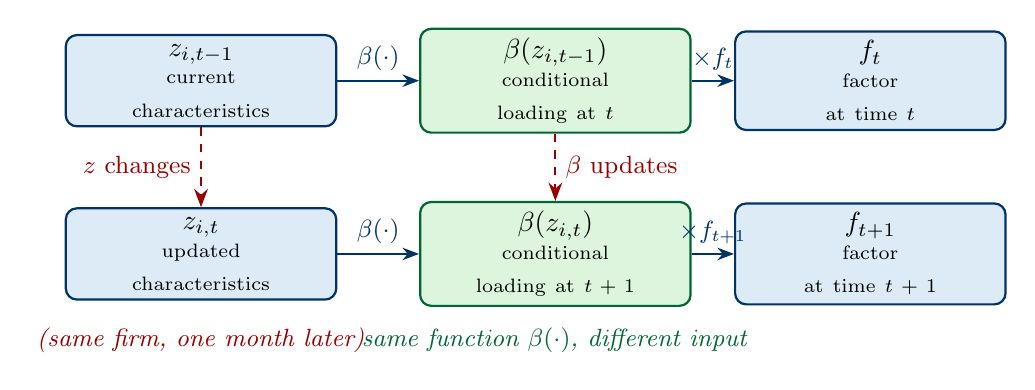
\begin{tikzpicture}[
  box/.style={rectangle, rounded corners, draw=darkblue, thick,
              fill=lightblue, text width=3.2cm, align=center,
              minimum height=1.1cm},
  wbox/.style={rectangle, rounded corners, draw=darkgreen, thick,
               fill=lightgreen, text width=3.2cm, align=center,
               minimum height=1.1cm},
  arrow/.style={-{Stealth[length=6pt]}, thick, darkblue},
  label/.style={font=\small\itshape, text=darkred, midway}
]

% left column: firm at time t-1
\node[box] (z1) at (0, 2.2) {$z_{i,t-1}$\\[2pt]\scriptsize current\\characteristics};
\node[box] (z2) at (0, 0.0) {$z_{i,t}$\\[2pt]\scriptsize updated\\characteristics};
\node[font=\small, darkred] at (0,-1.1) {\textit{(same firm, one month later)}};

% middle: beta function
\node[wbox] (beta1) at (4.5, 2.2) {$\beta(z_{i,t-1})$\\[2pt]\scriptsize conditional\\loading at $t$};
\node[wbox] (beta2) at (4.5, 0.0) {$\beta(z_{i,t})$\\[2pt]\scriptsize conditional\\loading at $t+1$};

% right: factor
\node[box] (f1) at (8.5, 2.2) {$f_t$\\[2pt]\scriptsize factor\\at time $t$};
\node[box] (f2) at (8.5, 0.0) {$f_{t+1}$\\[2pt]\scriptsize factor\\at time $t+1$};

% arrows
\draw[arrow] (z1) -- node[above, font=\small]{$\beta(\cdot)$} (beta1);
\draw[arrow] (z2) -- node[above, font=\small]{$\beta(\cdot)$} (beta2);
\draw[arrow] (beta1) -- node[above, font=\small]{$\times f_t$} (f1);
\draw[arrow] (beta2) -- node[above, font=\small]{$\times f_{t+1}$} (f2);

% dashed arrow showing z changes
\draw[-{Stealth}, dashed, darkred, thick] (z1) -- node[left, font=\small, text=darkred]{$z$ changes} (z2);
\draw[-{Stealth}, dashed, darkred, thick] (beta1) -- node[right, font=\small, text=darkred]{$\beta$ updates} (beta2);

% same function label
\node[font=\small, text=darkgreen] at (4.5, -1.1)
  {\textit{same function $\beta(\cdot)$, different input}};

\end{tikzpicture}
\end{center}

\medskip
\textbf{Key structural assumption:} the mapping $\beta(\cdot)$ is the \textbf{same
function for all firms at all times}. Time variation in betas comes entirely from
time variation in characteristics.

\end{frame}
%
%..................................................................
%
\begin{frame}{Cross-Sectional and Time-Series Variation — Simultaneously}

The conditional model captures \textbf{two sources of variation} with one object:

\bigskip
\begin{columns}
\begin{column}{0.48\textwidth}
  \begin{block}{Cross-sectional variation (same $t$)}
    At any given month, two firms with \textbf{different} $z_{i,t-1}$ get
    \textbf{different} betas:
    $$z_{A,t-1} \neq z_{B,t-1} \Rightarrow \beta_A \neq \beta_B$$
    Example: a small-cap and a large-cap in the same month have different
    market beta exposures.
  \end{block}
\end{column}
\begin{column}{0.48\textwidth}
  \begin{block}{Time-series variation (same firm)}
    For a single firm, betas change over time as its characteristics evolve:
    $$z_{i,t-1} \neq z_{i,s-1} \Rightarrow \beta_{i,t} \neq \beta_{i,s}$$
    Example: the same firm has a different beta when it is financially
    distressed vs.\ when it is healthy.
  \end{block}
\end{column}
\end{columns}
\end{frame}
%
%..................................................................
%
\begin{frame}{Cross-Sectional and Time-Series Variation — Simultaneously}
\begin{alertblock}{Contrast with static models}
\begin{center}
\begin{tabular}{lcc}
\toprule
& \textbf{Cross-sectional} & \textbf{Time-series} \\
\midrule
Static (FF, PCA) & \textcolor{darkgreen}{\checkmark} (different $\beta_i$ per firm) & \textcolor{darkred}{$\times$} (constant) \\
Conditional      & \textcolor{darkgreen}{\checkmark} & \textcolor{darkgreen}{\checkmark} \\
\bottomrule
\end{tabular}
\end{center}
\end{alertblock}

\end{frame}
%
%..................................................................
%
\begin{frame}{The Open Question: Choosing $\beta(\cdot)$}

The conditional factor model $r_{i,t} = \beta(z_{i,t-1})' f_t + u_{i,t}$ requires
specifying the function $\beta: \mathbb{R}^P \to \mathbb{R}^K$.

\bigskip
This is a \textbf{non-parametric estimation problem}: we have $n$ inputs and
need to learn a function from data.

\bigskip
\begin{center}
\begin{tabular}{p{2.8cm} p{3.8cm} p{4.2cm}}
\toprule
\textbf{Approach} & \textbf{Specification} & \textbf{Comment} \\
\midrule
\textbf{IPCA}
  & $\beta(z)' = z'\Gamma$, \quad $\Gamma \in \mathbb{R}^{P\times K}$
  & Simple, closed-form; misses nonlinear interactions \\[8pt]
\textbf{CA0}
  & Single linear layer
  & Equivalent to IPCA \\[8pt]
\textbf{CA1}
  & 1 hidden layer (ReLU)
  & Captures pairwise interactions \\[8pt]
\textbf{CA2}
  & 2 hidden layers (ReLU)
  & Richer nonlinearities \\[8pt]
\textbf{CA3}
  & 3 hidden layers (ReLU)
  & Maximum flexibility \\
\bottomrule
\end{tabular}
\end{center}
\end{frame}
%
%..................................................................
%
\begin{frame}{The Open Question: Choosing $\beta(\cdot)$}
\begin{exampleblock}{Why nonlinearity?}
Leading structural models (Campbell--Cochrane 1999, Bansal--Yaron 2004,
He--Krishnamurthy 2013) all predict that the mapping from state variables to betas
is \textbf{inherently nonlinear}. Linearity is a computational convenience, not a
theoretical prediction.
\end{exampleblock}

\end{frame}
%
%..................................................................
%
\begin{frame}{Nonlinear Effects That IPCA Cannot Capture}

\begin{center}
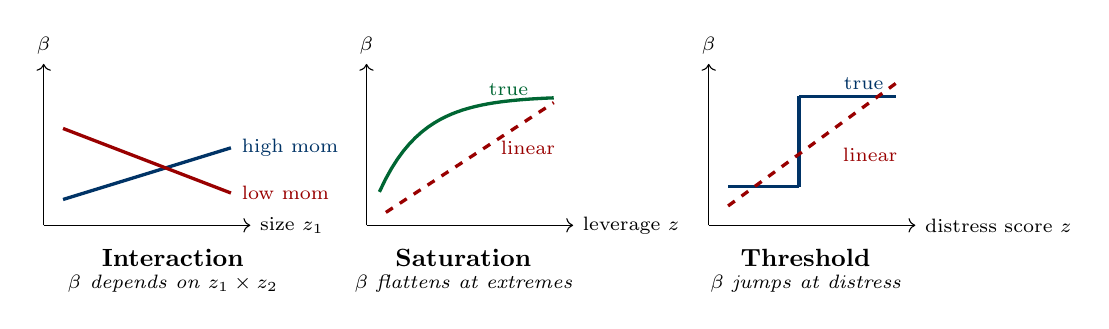
\begin{tikzpicture}[scale=0.82]

% Panel 1: interaction
\begin{scope}[xshift=0cm]
  \draw[->] (-1,0) -- (2.2,0) node[right,font=\scriptsize]{size $z_1$};
  \draw[->] (-1,0) -- (-1,2.5) node[above,font=\scriptsize]{$\beta$};
  \draw[darkblue, very thick] (-0.7,0.4) -- (1.9,1.2)
    node[right,font=\scriptsize,text=darkblue]{high mom};
  \draw[darkred, very thick] (-0.7,1.5) -- (1.9,0.5)
    node[right,font=\scriptsize,text=darkred]{low mom};
  \node[font=\small\bfseries] at (1.0,-0.5) {Interaction};
  \node[font=\scriptsize\itshape] at (1.0,-0.9)
    {$\beta$ depends on $z_1 \times z_2$};
\end{scope}

% Panel 2: saturation
\begin{scope}[xshift=4.0cm]
  \draw[->] (0,0) -- (3.2,0) node[right,font=\scriptsize]{leverage $z$};
  \draw[->] (0,0) -- (0,2.5) node[above,font=\scriptsize]{$\beta$};
  \draw[darkgreen, very thick, domain=0.2:2.9, samples=30]
    plot (\x, {2.0*(1 - exp(-1.5*\x))});
  \draw[darkred, dashed, very thick] (0.3,0.2) -- (2.9,1.9);
  \node[font=\scriptsize, text=darkgreen] at (2.2,2.1) {true};
  \node[font=\scriptsize, text=darkred] at (2.5,1.2) {linear};
  \node[font=\small\bfseries] at (1.5,-0.5) {Saturation};
  \node[font=\scriptsize\itshape] at (1.5,-0.9)
    {$\beta$ flattens at extremes};
\end{scope}

% Panel 3: threshold
\begin{scope}[xshift=9.3cm]
  \draw[->] (0,0) -- (3.2,0) node[right,font=\scriptsize]{distress score $z$};
  \draw[->] (0,0) -- (0,2.5) node[above,font=\scriptsize]{$\beta$};
  \draw[darkblue, very thick] (0.3,0.6) -- (1.4,0.6);
  \draw[darkblue, very thick] (1.4,0.6) -- (1.4,2.0);
  \draw[darkblue, very thick] (1.4,2.0) -- (2.9,2.0);
  \draw[darkred, dashed, very thick] (0.3,0.3) -- (2.9,2.2);
  \node[font=\scriptsize, text=darkblue] at (2.4,2.2) {true};
  \node[font=\scriptsize, text=darkred] at (2.5,1.1) {linear};
  %\draw[dashed, gray] (1.4,0) node[below,font=\scriptsize]{threshold}
    -- (1.4,0.6);
  \node[font=\small\bfseries] at (1.5,-0.5) {Threshold};
  \node[font=\scriptsize\itshape] at (1.5,-0.9)
    {$\beta$ jumps at distress};
\end{scope}

\end{tikzpicture}
\end{center}

\bigskip
\begin{alertblock}{IPCA assumes linearity in all three panels}
The dashed lines show what IPCA fits. The solid curves show what the true
relationship might look like. Neural networks can approximate all three patterns.
\end{alertblock}

\end{frame}
%
%..................................................................
%
\begin{frame}{Summary: The Role of Characteristics}

\begin{center}
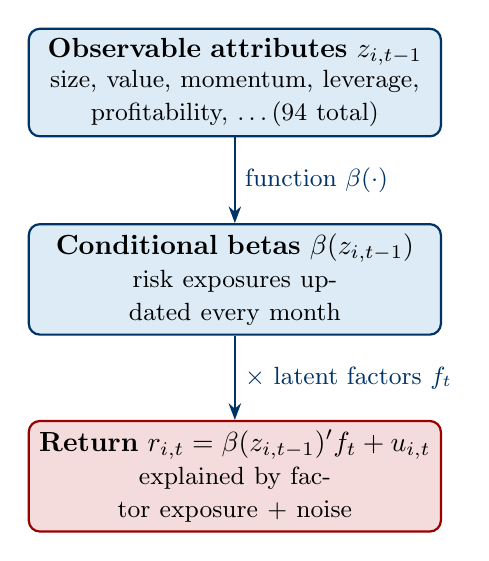
\begin{tikzpicture}[
  box/.style={rectangle, rounded corners, draw=darkblue, thick,
              fill=lightblue, text width=5cm, align=center, minimum height=1cm},
  abox/.style={rectangle, rounded corners, draw=darkred, thick,
               fill=lightred, text width=5cm, align=center, minimum height=1cm},
  gbox/.style={rectangle, rounded corners, draw=darkgreen, thick,
               fill=lightgreen, text width=11cm, align=center, minimum height=1cm},
  arrow/.style={-{Stealth[length=6pt]}, thick, darkblue}
]
\node[box] (obs) at (0, 5.0)
  {\textbf{Observable attributes} $z_{i,t-1}$\\
   \small size, value, momentum, leverage,\\profitability, \ldots (94 total)};

\node[box] (beta) at (0, 2.5)
  {\textbf{Conditional betas} $\beta(z_{i,t-1})$\\
   \small risk exposures updated every month};

\node[abox] (ret) at (0, 0.0)
  {\textbf{Return} $r_{i,t} = \beta(z_{i,t-1})'f_t + u_{i,t}$\\
   \small explained by factor exposure + noise};

\draw[arrow] (obs) -- node[right, font=\small]{function $\beta(\cdot)$} (beta);
\draw[arrow] (beta) -- node[right, font=\small]{$\times$ latent factors $f_t$} (ret);

\end{tikzpicture}
\end{center}
\end{frame}
%
%..................................................................
%
\begin{frame}{Summary: The Role of Characteristics}
\begin{columns}
\begin{column}{0.48\textwidth}
  \textbf{What characteristics provide:}
  \begin{itemize}
    \item Real-time, firm-specific risk information
    \item Cross-sectional differentiation
    \item Time-series updating without re-estimation
    \item A high-dimensional input for the beta network
  \end{itemize}
\end{column}
\begin{column}{0.48\textwidth}
  \textbf{The remaining question:}\\
  What is the function $\beta(\cdot)$?
  \begin{itemize}
    \item IPCA: linear ($\beta = \Gamma'z$) — simple but restrictive
    \item Conditional Autoencoder: neural network — flexible, nonlinear
    \item Theory predicts nonlinearity; data confirms it
  \end{itemize}
\end{column}
\end{columns}

\end{frame}

\end{document}
